\chapter{Modelling}
\label{chap:modelling}


\begin{quote}
    \textit{All models are wrong, but some are useful.} \\
    - George Box \cite{box1976science}.
\end{quote}

Models of the state of the ocean can vary from simple relation between variables, such as in \textcite{zhang2019autonomous} to spatiotemporally evolving, first-principles based models such as the Regional Ocean Modeling System (ROMS) \cite{shchepetkin2005regional}. As the complexity of the model increases, so does the computational effort needed to update and propagate it, thus, there exists an upper limit to the complexity of on board models in marine robotics. In this chapter, common models and methods for modelling in adaptive sampling with underwater robots are presented along with examples from the literature. The main focus will be on statistical models and \textit{subsumption-based} \cite{brooks1986robust} solutions for modelling or estimating the decision variables. Having a model of the environment makes taking informed decisions easier, and thus the model should be designed with that in mind. A statistical model can estimate a measurement value at an unvisited position in time and space with a certain (un)certainty. Without an on-board model all decisions made on board the robot become myopic, and this can lead to exploring and getting stuck at local maxima, as presented in \textcite{hwang2019auv}. It needs to be specified that the model need not be of the environment it self, but it can also be of the data collected, vehicle state or perceived risk, depending on the goal of the adaptive behavior.  

\section{Subsumption-based models}
\textcolor{red}{Heavily on examples from Zhang – purpose driven methods with clear scientific goal in mind
}
\begin{quote}
    \textit{subsume} - verb: To include or place within something larger or more comprehensive : encompass as a subordinate or component element.
\end{quote}




\subsection{Rule based}
\textit{Ad hoc}, rule based, or \textit{subsumption} based models can be more intuitive than the models based on spatial statistics, however, they can can be just as effective in collecting the desired data. The \textit{subsumption} based model is often formulated as a finite state machine or rule-based expert system. In this section some \textit{subsumption} based models and is presented, starting with the upwelling front detection model presented in \textcite{zhang2012autonomous,zhang2016autonomous}, continuing with the vertical models presented in \textcite{zhang2011peak,zhang2019autonomous} and finally looking at the front model in \textcite{fossum2021adaptive}.These models or behaviors are reactionary patterns programmed using expert field knowledge of the phenomena that one wants to sample. 



The problem definition of any planning algorithm for adaptive sampling used here is as follows: "based on current observations and models, what should the robot do \textit{now}?". 

Subsumption architectures \cite{fossum2019adaptive}, or \textit{ad hoc} behaviors, are a set of behaviors defined by a \textit{Sense\textrightarrow Act} strategy, where the model is baked into the assumptions of the behavior. The behavior in such a method must be customized for the purpose, and is generally not equipped to handle unexpected events. Implementation of subsumption architectures are usually done as a finite state machine, such as is presented in \textcite{fossum2021adaptive}. The "\textit{planning}" done in these architectures lies in the rule-based behavior, and depends on the internal state of the AUV. This does not mean that they are not useful, and generally they are more intuitive than information-theoretic approaches. 

\subsubsection*{Crossing the Polar Front}
In \textcite{fossum2021adaptive}, a state machine for front crossing is presented, where if the AUV crosses a certain temperature threshold, the front is considered to be crossed. The AUV is programmed to cross the front in a zigzag manner, where if the front is not detected after a set number of attempts, a "regain front" maneuver is initiated. This method is quite similar to the algorithm presented in \textcite{zhang2016autonomous}. The polar front was also crossed adaptively by LAUV Harald in February 2021, as presented in \textbf{paper A}. 


\subsubsection*{Vertical Feature Tracking}
It is possible to relate two strongly correlated features, in \textcite{zhang2011peak}, a strong horizontal auto correlation of the CDOM measured by the AUV is assumed. Where the AUV captures the depth of the CDOM max during decent and closes a sampling bottle at that depth during ascent. In \textcite{zhang2019autonomous}, the temperature at the \acrfull{scm} is detected, and followed for continuous sampling of the \acrshort{scm}, while executing a pseudo-lagreangian drift, drifting with the current in the horizontal plane. This relies on the assumption that by locking on to an isotherm, the AUV stays in to that water-mass, and thus also the \acrshort{scm}. 


\subsubsection*{Upwelling Front Crossing}
Another front crossing algorithm, presented in \cite{zhang2012autonomous,zhang2013two,zhang2016autonomous}, was also implemented as a finite state machine. The algorithm used the difference in temperature across one dive or ascent to assess the vertical variance in the water column, thus determining if the AUV was in upwelled mixed water or in stratified, non-upwelled water. 
\subsubsection*{Bio-inspired}
While the state machine approach provides a sequential architecture for decision making, one can also implement bio-inspired continuous reaction patterns, these behaviors are  often described as inspired by biology, such as the crustacean-inspired behavior described in \cite{hwang2019auv}, used to move the agent towards higher salinity.  


\subsubsection*{Parsimony}
When modeling, it is important to take into consideration the complexity of the model, and the data used to generate it. A complex model, trying to explain the minutia of an ocean phenomena might be prone to overfitting, and vice versa. The goal is to describe the desired phenomena, while having a model that is simple; the parsimonious model. One way of obtaining this model is to use only informative samples, this can be of special importance when dealing with large data sets. Methods for dealing with large data sets are presented in \textcite{rasmussen2003gaussian}. This challenge is also addressed in \textcite{fossum2019adaptive}, where it is termed as the optimally vs. computability trade-off, meaning that there can exist an optimal solution or model that is not computationally tractable.

\subsubsection*{Smoothness}
In \cite{eidsvik2015value}, the point is made that a map generated from a GP is not representative for the features found in the real data, but the predictive mean of the data. The map generated by a GP is generally smoother than the real data, due to smoothing effect from the covariance functions. \textit{"Kriging maps deliver an incorrect sense of spatial continuity" \cite{eidsvik2015value}} One can implement non-smooth covariance functions, such as the Matèrn kernel with $\nu=1/2$, however, this is not common. The reader is reminded of the inequality $E(f(\mathbf{y})) \neq f(E(\mathbf{y}))$, and warned against using the predictive mean for feature generation. 

\subsubsection*{Temporal modeling}
In the literature investigated, the ocean/water is either assumed to be static, \textcite{kemna2018multi,stankiewicz2021adaptive}, or the temporal effects are simplified to white noise; adding noise to the measurement, dependent on the age of the measurement, such as in \textcite{fossum2019adaptive}. The assumption behind this is often that \textit{robot speed $>>$ process speed}, and the example given in \textcite{fossum2018information} is \textit{robot speed $= u_r = 1.5m/s$} and \textit{current speed $ = u_c = 0.2 m/s$}. It is of the authors opinion that this is a false dichotomy, since the current is moving in an (on average) uniform direction, and the robot often is attempting to sample a volume or area. Using the values above, we can see that in the time it would take to traverse the perimeter of a square with the robot, $100\% \frac{4\cdot0.2 m/s}{1.5 m/s} = 53.3\%$ of the water inside the square would have been advected. Thus, the noise added from the age of the measurement must reflect this degradation in signal. An alternative is to model the temporal effects. Recent efforts \cite{berget2022adaptive} have attempted to address this problem with an advection-diffusion \acrfull{spde} model, where the advection  and diffusion of the field is modelled. The training data for this model, comes from a numerical ocean model, increasing the risk of overfitting without bounding it with measurement data. 

\section{Statistical models}
Statistical modeling affords deliberation on different potential outcomes, enabling optimization over the predicted outcome space. Apart from the above mentioned advection-diffusion \acrshort{spde}-model, the preferred\cite{low2009multi,kemna2016adaptive,kemna2018multi,fossum2018information,fossum2019toward,stankiewicz2021adaptive,berget2018adaptive}, and \textbf{papers B, C, D, F, and E} data driven model is the \acrfull{gp}. 

\subsection{Noise}
\label{sec:noise}
In statistical modelling, there will always be noise and in this section, two types of noise will be addressed, sensor noise and process noise. Sensor noise is the noise inherent to the method of measuring a parameter. 
\subsubsection*{Sensor noise}
Usually, sensor noise has a known distribution, as sensors used in the ocean are calibrated from the manufacturer. While salinity and temperature measurements usally \textcolor{red}{TODO}

\subsection{Gaussian Process}
The \acrshort{gp} model is covered in much of the literature, here the notation from \cite{rasmussen2003gaussian} is used and presented along with elements from \cite{eidsvik2015value} and \cite{cressie2015statistics}. In order to tie it to the underwater sampling domain, the modeling done by \cite{fossum2019adaptive}, \cite{kemna2018multi} and \cite{stankiewicz2021adaptive} is presented in the relevant sections. From  \textcite{rasmussen2003gaussian}:
\begin{quote}
    \textit{A Gaussian Process is a collection of random variables, any number of which have a joint Gaussian distribution. }
\end{quote}
The GP can be described by the mean function $m(\mathbf{x})$ and the covariance function, or kernel $k(\mathbf{x},\mathbf{x}')$, of a real process $f(\mathbf{x})$, and written as in Equation \eqref{eq:mod_gp}, where $\mathbf{x}$ is a vector of locations. In \textcite{cressie2015statistics} $\mathbf{x}$ is presented as functions of locations, $\mathbf{s}$, ($\mathbf{x}(\mathbf{s})$), however, this function is moved to $m(\cdot)$ in \textcite{rasmussen2003gaussian}. 

\begin{align}
\label{eq:mod_gp}
    f(\mathbf{x}) = \mathcal{GP}(m(\mathbf{x}),k(\mathbf{x},\mathbf{x}'))
\end{align}


While \textcite{rasmussen2003gaussian} is founded in the machine learning space, \textcite{cressie2015statistics} and \textcite{eidsvik2015value} are situated in the geostatistics domain, their fundamentals for spatial GPs are quite similar. Both considers the possibility of noisy measurements, CW considers this noise as a combination of the \textit{nugget effect} (from gold-mining, discrete spatial events with no spatial correlation) and measurement noise, whereas Rasmussen is more generic in their approach. The measurement model then becomes as presented in Equation \eqref{eq:mod_meas} and the prior on the noisy observations, $y$, become as in Equation \eqref{eq:mod_cov}, where $\delta_{pq}$ is a Kronecker delta which is one if and only if $p=q$.
\begin{align}
    \label{eq:mod_meas}
    y &= f(\mathbf{x}) + \varepsilon \text{, where} \\ 
    \varepsilon &\sim \mathcal{N}(0,\sigma_n^2) \\ 
    \label{eq:mod_cov}
    cov(y_p,y_q) &= k(\mathbf{x}_p,\mathbf{x}_q) + \sigma_n^2 \delta_{pq}
\end{align}

The predictive equations for a GP as described in Rasmussen are presented in Equation \eqref{eq:mod_gp_pred}, where $\mathbf{f}_*$ is the prediction, $X$ is the sites of the measurements, $\mathbf{y}$, $X_*$ are the prediction sites, $K(A,B)$ is the covariance matrix for sites in $A$ and $B$ and $\Bar{\mathbf{f}}_*$ is the predictive mean.  

\begin{align}
    \label{eq:mod_gp_pred}
    \mathbf{f}_*|X,\mathbf{y},X_* &\sim \mathcal{N}(\Bar{\mathbf{f}}_*,cov(\mathbf{f}_*))\text{, where} \\ 
    \label{eq:mod_gp_pred2}
    \mathbf{\mu} = \Bar{\mathbf{f}}_* &\triangleq \mathbb{E}[\mathbf{f}_*|X,\mathbf{y},X_*] = K(X_*,X)[K(X,X)+\sigma_n^2 I]^{-1}\mathbf{y} \\
    \label{eq:mod_gp_pred3}
    \Sigma = cov(\mathbf{f}_*) &= K(X_*,X_*) - K(X_*,X)[K(X,X)+\sigma_n^2 I]^{-1}K(X,X_*)
\end{align}


Rasmussen assumes zero mean, while in CW, the formulation differs for the predictive mean in Equation \eqref{eq:mod_gp_pred3}, adding the predictive function $m(X_*)$ and the error, $\mathbf{y} - m(X)$ as a gain in stead of $\mathbf{y}$. This gives the flexibility that $\mathbf{y} - m(X)$ needs to be Gaussian, in stead of $\mathbf{y}$ needing to be Gaussian.  


\subsection{Covariance structures}
\textcolor{red}{variograms, kernel functions, horizontal vs vertical de-correlations, Eidsvik, Rasmussen, Cressie}

Covariance functions, or kernels, $\mathbf{k}(\cdot,\cdot)$, describe how measurements correlate, and the choice of kernel is of utmost importance to the final model. The covariance function can be analytical or empirical, the analytical covariance functions relevant for oceanic adaptive sampling will be presented. The most common kernel for spatial data is the squared exponential (SE), also known as the radial basis function or Gaussian kernel, presented in Equation \eqref{eq:mod_kernel_se} and Figure \ref{fig:kernels}, where $l$ is the characteristic length scale and $\sigma_f^2$ is the process noise. The characteristic length, $l$, is also known as the \textit{de-correlation length} and the \textit{length-scale}. 

\begin{align}
\label{eq:mod_kernel_se}
    k_{SE}(r) &= \sigma_f^2 exp\Big(\frac{-r^2}{2 l^2}\Big)\\
    r &= |x_p-x_q|
\end{align}

The SE kernel is invariant to $x_p$ or $x_q$, and isotropic, it was used by \textcite{kemna2018multi}, \textcite{stankiewicz2021adaptive} in their GP models. \textcite{rasmussen2003gaussian} mentions critique against the SE kernel for being overly smooth, an effort to remedy this is done by the Matérn kernel in Equation \eqref{eq:mod_kernel_matern}, with positive parameters $\nu$ and $l$ and where $K_{\nu}$ is the modified Bessel function of the second kind \cite{abramowitz1965handbook}, and $\Gamma(n) = (n-1)!$. 

\begin{align}
    \label{eq:mod_kernel_matern}
    k_M(r) = \frac{2^{1-\nu}}{\Gamma(\nu)} \Big(\frac{\sqrt{2\nu}r}{l}\Big)^{\nu} K_{\nu} \Big(\frac{\sqrt{2\nu}r}{l}\Big)
\end{align}

Equation \eqref{eq:mod_kernel_matern} becomes simpler when $\nu$ is half integer: $\nu = p + 1/2$, where $p$ is a non-negative integer, the simplification is presented in (\ref{eq:mod_kernel_matern_simple}).
\begin{align}
    \label{eq:mod_kernel_matern_simple}
    k_{\nu = p + 1/2} (r) = exp\Big(-\frac{\sqrt{2\nu }r}{l}\Big)\frac{\Gamma(p+1)}{\Gamma(2p+1)}\sum_{i=0}^p \frac{(p+1)!}{i!(p-i)!}\Big(\frac{\sqrt{8\nu}r}{l}\Big)^{p-i}
\end{align}
The special case of $p=1$ was used by  \textcite{fossum2018information,fossum2019toward,fossum2019adaptive} and \textcite{berget2018adaptive}, presented in Equation \eqref{eq:mod_kernel_matern_1}, with keeping the notation from \textcite{rasmussen2003gaussian}. 

\begin{align}
\label{eq:mod_kernel_matern_1}
    k_{\nu=3/2}(r) = \Big(1 + \frac{\sqrt{3}r}{l}\Big)exp\Big(-\frac{\sqrt{3}r}{l}\Big)
\end{align}
Other kernels worth mentioning, but without examples from oceanic adaptive sampling are the Exponential kernel, presented in Equation \eqref{eq:mod_kernel_gauss} \cite{eidsvik2015value}, and the Cauchy type kernel presented in Equation \eqref{eq:mod_kernel_cauchy}. 
\begin{align}
    \label{eq:mod_kernel_gauss}
    k_E(r) &= \sigma_f^2 exp\Big(-\frac{r}{l}\Big) \\ 
    \label{eq:mod_kernel_cauchy}
    k_C(r) &= \sigma_f^2 exp\Big(-\frac{1}{(1+r/l)^3}\Big)
\end{align}

All kernels can be expanded to $\mathbb{R}^n$, an example of the SE kernel is presented in Equation \eqref{eq:mod_kernel_multi}, where $M$ is a symmetric matrix. Possible choices for M presented in \eqref{eq:mod_m} where $\mathbf{l}$ is a vector of positive values and $\Lambda$ is a $D\times k$ matrix, $k<D$.

\begin{align}
\label{eq:mod_kernel_multi}
    k(\mathbf{x}_p,\mathbf{x}_q) = \sigma_f^2 exp\Big(-\frac{1}{2}(\mathbf{x}_p-\mathbf{x}_q)^{\intercal}M (\mathbf{x}_p-\mathbf{x}_q) \Big)\\ 
    \label{eq:mod_m}
    M_1 = l^{-2}I, \hspace{20pt} M_2 = diag(\mathbf{l})^{-2}, \hspace{20pt} M_3 = \Lambda \Lambda^{\intercal} + diag(\mathbf{l})^{-2} 
\end{align}


Finally, one can combine kernels to make new kernels, both by taking the product, $k(\mathbf{x},\mathbf{x}')=k_1(\mathbf{x},\mathbf{x}')k_2(\mathbf{x},\mathbf{x}')$, or by summing, $k(\mathbf{x},\mathbf{x}')=k_1(\mathbf{x},\mathbf{x}')+k_2(\mathbf{x},\mathbf{x}')$, two kernels. When the kernel composition has been decided, the parameters of the kernel (hyperparameters, e.g. $\mathbf{\theta} = (M,\sigma_f^2)^{\intercal}$ for Equation \eqref{eq:mod_kernel_multi}) have to be ascertained.

\subsubsection*{Hyperparameter Estimation}
There are two approaches to ascertain the hyperparameters of a GP, the first is from geoscience and is termed a variogram, and the second is from machine learning and is better described as model fitting. The two are concerned with the same problem, for the most intuitive approach, the variogram is presented first. An empirical variogram can be computed from the data as in Equation \eqref{eq:mod_variogram}, where $T(h)$ is a small tolerance region around $h$.

\begin{align}
    \label{eq:mod_variogram}
    2\Hat{\gamma}_y^0 (h) \equiv ave\{(y(x_i)-y(x_j))^2:||x_i-x_j|| \in T(h);i,j=1,\ldots,m \}
\end{align}

For Equation \eqref{eq:mod_variogram} to be an appropriate estimator for $2\gamma_f(\cdot)$, an assumption of isotropy has to be made: $2\gamma_f(\mathbf{h}) = 2\gamma_f^0(||\mathbf{h}||)$. In addition, the measurement noise, $2\sigma_{\varepsilon}^2$ has to be subtracted from Equation \ref{eq:mod_variogram}. If the measurement noise is unknown, it is inseparable from the nugget effect, \textcite{rasmussen2003gaussian} does not separate the measurement noise and nugget, while \textcite{cressie2015statistics} and \textcite{eidsvik2015value} does. An example semivariogram (in the variogram, measurements are counted twice; $(y(x_i)-y(x_j))^2 = (y(x_j)-y(x_i))^2$, thus we use the half variogram) is presented in Figure \ref{fig:mod_variogram}. In the figure, a kernel function is fitted to the experimental data, minimizing the Mean Squared Prediction Error (MSPE). 

\begin{figure}
    \centering
    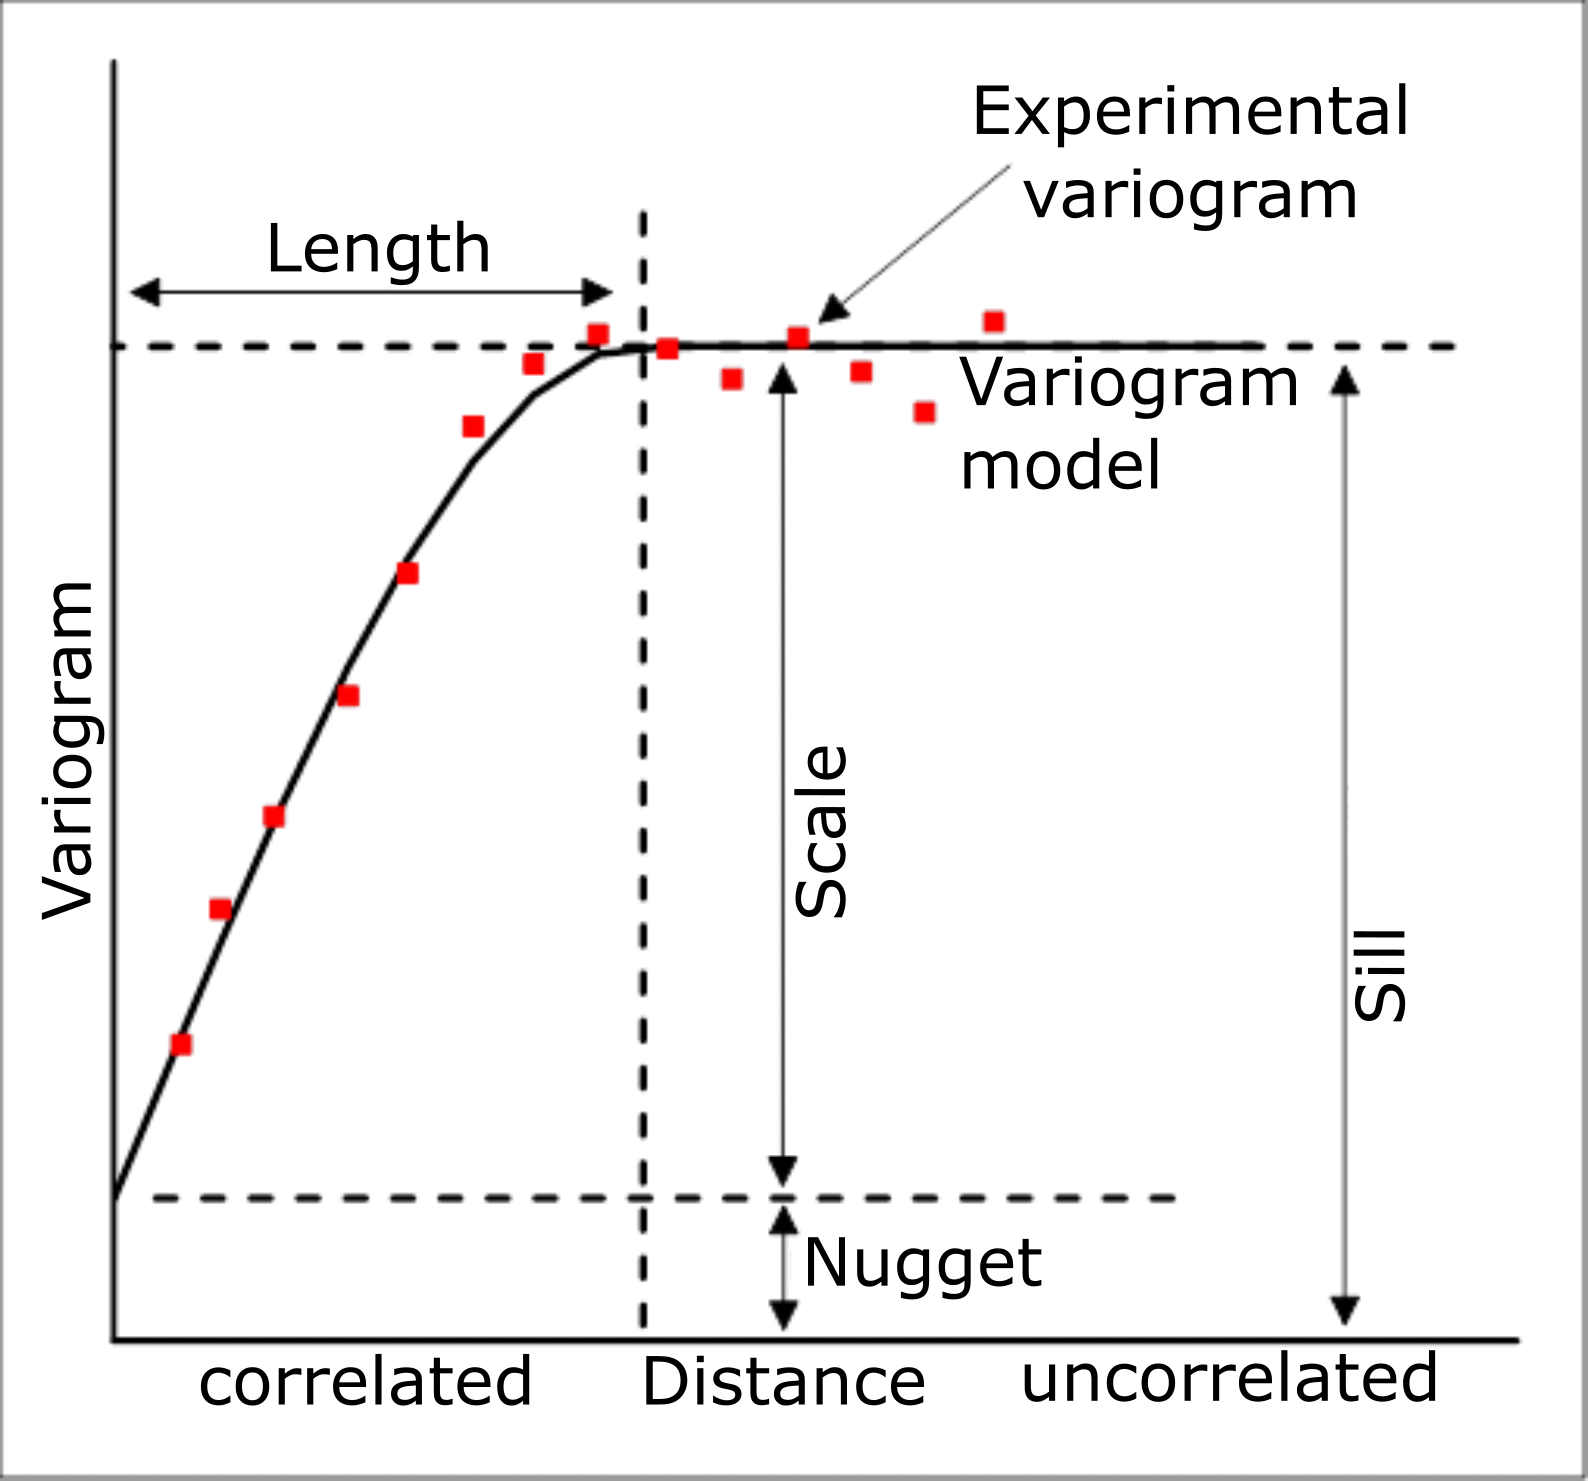
\includegraphics[width=0.9\textwidth]{figures/expvariogram.png}
    \caption{Experimental semivariogram, where the red dots are the empirical semivariogram, $\hat{\gamma}_y^0(h)$, the nugget (and measurement noise), $\sigma_n^2$ is the discontinuity at $h=0$, length is indicated; correlated with the length scale, the exponential kernel is fitted to $\hat{\gamma}_y^0(h)$, and the total variance, $Sill = \sigma_n^2 + \sigma_f^2$, is also indicated. Figure modified, from \textit{Visual Sample Plan from Pacific Northwest National Laboratory.}}
    \label{fig:mod_variogram}
\end{figure}

\begin{figure}
    \centering
    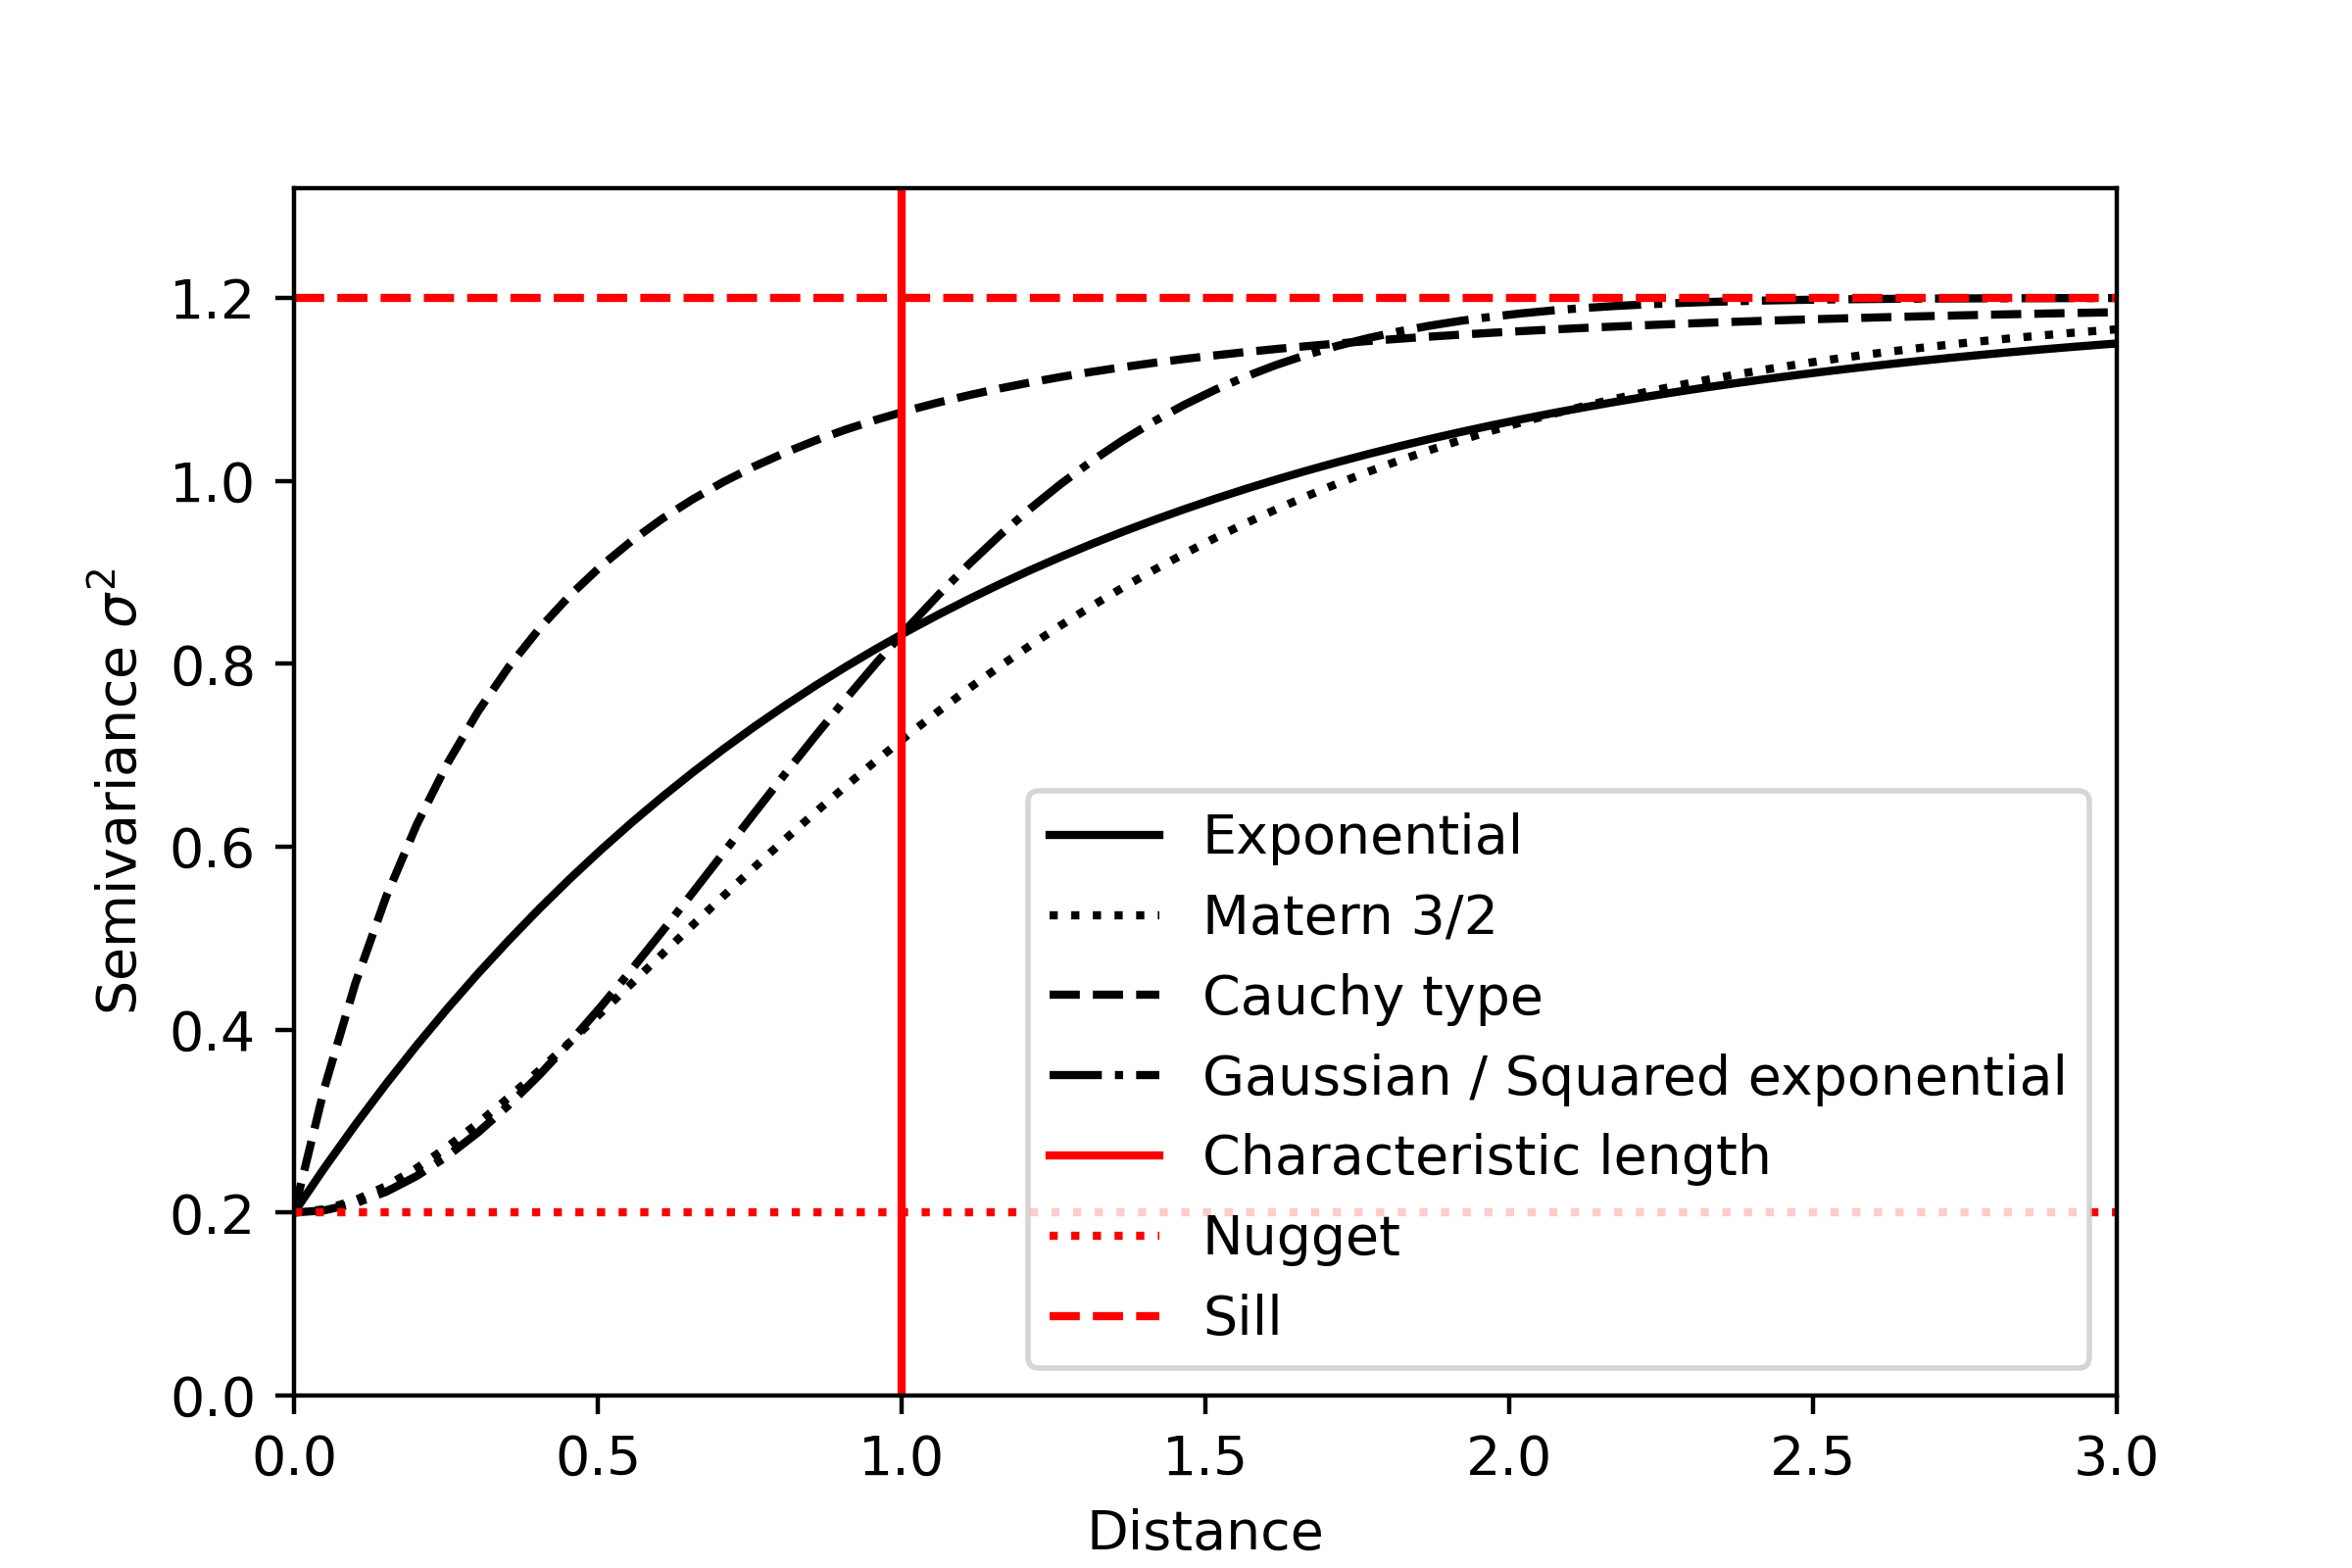
\includegraphics[width=0.9\textwidth]{figures/kernels.png}
    \caption{Semivariograms from exponential, Matérn 3/2, Cauchy type and Gaussien kernels, with nugget = $0.2$, sill = $1.0$, length scale = $1.0$, and scale = $1.0$.}
    \label{fig:kernels}
\end{figure}

In \textcite{fossum2018information}, a semivariogram from simulated data was used to set the length scale before sampling real data, while \cite{fossum2019toward} used a variagram from remote sensing data.  Another way of finding the hyperparameters, $\mathbf{\theta}$ is to follow the procedure of finding the log \textit{marginal likelihood}, presented in Equation \eqref{eq:mod_log_mar}, where $K_y=K_f+\sigma_n^2 I$.

\begin{align}
\label{eq:mod_log_mar}
    \text{log} p(\mathbf{y}|X,\mathbf{\theta}) = -\frac{1}{2}\mathbf{y}^{\intercal}K_y^{-1}\mathbf{y} -\frac{1}{2}\text{log}|K_y|-\frac{n}{2}\text{log}2\pi
\end{align}

The hyperparameters are then found by maximizing the (log) marginal likelihood, by partially differentiating (\ref{eq:mod_log_mar}) with respect to the hyperaparameters. The derivation is shown in \textcite{rasmussen2003gaussian}, chapter 5, and the expression is presented in Equation \eqref{eq:mod_log_diff}, where $\mathbf{\alpha} = K^{-1} \mathbf{y}$ and $K$ is the noise free (without nugget or measurement error, $\sigma_n^2$) covariance matrix. This method was used for hyperaparameter estimation by \textcite{stankiewicz2021adaptive}. 

\begin{align}
    \label{eq:mod_log_diff}
    \frac{\partial}{\partial \theta_j} \text{log}p(\mathbf{y}|X,\mathbf{\theta}) = \frac{1}{2}trace\Big((\mathbf{\alpha \alpha}^{\intercal} - K^{-1})\frac{\partial K}{\partial \theta_j}\Big)
\end{align} 

This method can be stuck at local maxima, depending on the search strategy applied an the structure of the data. One way to avoid this is to restart the optimization at different points in the input space, choosing the "best" solution from all iterations. 


\subsection{Prior}
\label{sec:prior}

The \textit{prior probability distribution} or \textit{prior} is our best estimate, or guess of a parameter and its distribution before we have measured it. The prior can be generated in several ways and here we present some common modes of generating a prior in adaptive sampling in the marine domain. First, the naive or \textit{uninformative} \cite{gelman1995bayesian} prior is presented, followed by the in-situ prior, remote sensing prior, scenario based and simulation model based prior. 

\subsubsection{The naive approach}
The naive approach is the simplest, but also least informative prior. Here the prior belief is that we do not know anything about the parameter we are about to measure or its distribution. These priors can be useful in situations where there is no previous data available or when the prior is not of interest. One such case is presented in \textbf{paper F}, where the model is initiated with high uncertainty and no estimate. 

\subsubsection{Pilot Survey}
The \textit{in-situ} prior, or pilot survey, is gained by running a predefined sampling scheme before building a prior from the data. In \cite{kemna2018multi} (chapter 8) a method for designing a pilot survey over a predefined area is presented, where the survey can be weighted from maximizing the distance between the waypoints to random sampling. The maximum distance case can be found by maximizing utility function \textit{D} presented in Equation \ref{eq:prior_dist}, which calculates the minimum distance between waypoints, $\mathbf{x}$, and previously visited paths, $S$. 

\begin{align}
    \label{eq:prior_dist}
    D(\mathbf{x}_i) = min(d(\mathbf{x}_i,s_j))\hspace{5pt},\hspace{5pt} \forall s_j \in S
\end{align}

This approach applied to a rectangular survey area in $\mathcal{R}^2$ will result in a cross-pattern, using the corners of the area as waypoints. In order to weigh in random sampling a "temperature"-factor, $\tau$, is introduced and the probability of choosing a waypoint is calculated using the softmax-equation \cite{sutton1998introduction} in Equation \ref{eq:prior_softmax}. 
\begin{align}
    \label{eq:prior_softmax}
    p(\mathbf{x}_i) = \frac{e^{D(\mathbf{x}_i)/\tau}}{\sum_j e^{D(\mathbf{x}_j)/\tau}}
\end{align}

Letting $\tau \rightarrow \infty$ will result in choosing random waypoints, and setting $\tau = 1$ will give the same result as without the softmax function, and \cite{kemna2018multi} recommends using $\tau = 6$ for the most stable performance. 

The pilot survey approach was also used by \textcite{fossum2019toward}, where an AUV was programmed to undulate in a yoyo-pattern around the perimiter of the operational area. The pilot survey approach can be used to capture maxima in the vertical direction \cite{zhang2011peak,zhang2019autonomous}, using an AUV. In \textcite{zhang2011peak} the depth of the maximum CDOM fluorescence was found and used for triggering an on board water sampler, whereas in \textcite{zhang2019autonomous}, the deep chlorophyll-a max (DCM) was found and associated with an isotherm for easier long-term tracking. 


\subsubsection{External and Remote sensing prior}
As the name suggests, the external and remote sensing prior uses data from outside the robot sensors to obtain a prior estimate of the state of the ocean. Satellite data can give information about parameters in the sea surface, such as the Sea Surface Temperature (SST), phytoplankton blooms, turbidity and sea surface anomaly. The data gathered from a satellite can give a good overview over vast areas, but is prone to disturbance from clouds, and has a poor spatial (depending on the satellite) and temporal (one image per day) resolution compared to the AUV spatiotemporal reference frame. Another challenge with satellite data is the age of the data, as the images need to be downloaded to earth and distributed. An oft used external data source is shipboard sensors such as the Conductivity Temperature and Depth (CTD) that is lowered by winch from the ship in order to take a vertical profile, or the thermosalinograph, which is a CTD situated in the ferry-box, making continuous measurements near the surface. In \cite{fossum2021adaptive}, the approximate location of the arctic front in the Barents Sea was found using the on board CTD, before deploying the adaptive AUV mission. Data from satellites was used in \cite{fossum2019toward} in order to determine the \textit{characteristic length scale}.


\subsubsection{Simulation prior}
When generating a prior from simulation, the data from a simulated ocean environment, such as the ROMS model, is used and analyzed. In \cite{berget2018adaptive}, the output from the DREAM model was used to generate a prior, while in \cite{fossum2018information}, data from SINMOD was used to find the noise level and \textit{characteristic length scale}.

\subsubsection{Scenario prior}
A scenario prior is in reality a series of priors, or scenarios based on different criteria. These scenarios are often gathered from remote sensing or models, and in that sense they are in that category. The difference is that we have one or more informative variables that help us choose the correct prior or combination of priors for the time and place for sampling. One such informative variable may be wind speed and direction. In \cite{fossum2020compact}, different scenarios based on remote sensing data of the SST were classified, and served as a look-up table of scenarios, where the field of SST could be attempted reconstructed from a relatively small measurement from a surface craft. 

\subsubsection{Prior Function}
One can try and construct a function, $\hat{y} = m(\mathbf{x})$, that predicts the response variable, $\hat{y}$ from the input vector, $\mathbf{x}$. One common approximation of $m(\mathbf{x})$ is the linear combination $m(\mathbf{x}) = \mathbf{\beta x^{\intercal}}$, as presented in the Temperature over the Americas example in chapter 4 of \cite{cressie2015statistics}. Here, one can also construct input features, as was done in the example; $\mathbf{x} = [1,x_0, x_1,x_1^2, x_1^3]$, where $[x_0,x_1] = [lon,lat]$. The main goal of $m(\mathbf{x})$ is to make the residual $\Tilde{y} = f(\mathbf{x})-m(\mathbf{x})= y-\hat{y}$ as Gaussian as possible. 




\subsection{Non-Gaussian variables}
Some oceanic variables, such as chlorophyll a concentration are not Gaussian in their distribution, but log Gaussian. It is possible to construct a log-GP ($\ell$GP), where the measurement is modified before feeding it into the GP. In \cite{kemna2018multi} this is denoted as $\mathbf{z} = \text{ln} \mathbf{y}$, where the GP's posterior mean and variance $\Bar{\mathbf{f}}_*$ and $cov(\mathbf{f})$ are used to calculate the posterior mean and variance, as presented in (\ref{eq:mod_lgp1}) and (\ref{eq:mod_lgp2}). 
\begin{align}
    \label{eq:mod_lgp1}
    \Bar{\mathbf{f}}_{\mathbf{y}*} &= exp\Big(\Bar{\mathbf{f}}_* + \frac{cov(\mathbf{f})}{2}\Big) \\ 
    \label{eq:mod_lgp2}
    cov(\mathbf{f}_{\mathbf{y}}) &= \Bar{\mathbf{f}}_{\mathbf{y}*}^2(exp(cov(\mathbf{f})-1))
\end{align}

Furthermore, \textcite{eidsvik2015value}, chapter 4.5 presents methods for skew-normal models, where the Gaussian distribution is extended by enforcing skewness in a selected direction. It is also possible to construct a hierarchical model, to transform the data to responses that appear Gaussian, such as the $\ell$GP\cite{low2009multi,kemna2016adaptive} (\textbf{paper C}) or the square root transform. 

%\subsubsection*{Temporal modeling}
%The temporal aspect of Gaussian Process modeling is often assumed to be static\cite{fossum2018information,fossum2019toward,stankiewicz2021adaptive, kemna2018multi} (\textbf{papers A, B, \textcolor{red}{yaolin}), or simplified to white noise; adding noise to the measurement, dependent on the age of the measurement \textcite{fossum2019adaptive}. Another approach is to implement 


\subsection{Implementations}
In the literature and papers included, there are some flavours of implementations of the \acrshort{gp}, depending on the underlying assumptions and the available data. Implementations where a static field is assumed\cite{low2009multi,kemna2016adaptive,fossum2019toward}, such as in \textbf{paper  \textcolor{red}{yaolin}} tend to use the previous output of the \acrshort{gp} as their prior and ingesting the latest measurements as they come in. Other implementations evaluate the entire set of measurements in the prediction, using a de-trending function as a prior and adding temporal noise to the measurements, as presented in \textbf{papers B and C}. Temporal effects are also accounted for by a 2D \acrshort{spde}-model\cite{berget2022adaptive}, estimating the flow and diffusion in the data field. 

While a \acrshort{gp} can be evaluated at any location in the input space, most implementations use a gridded approach\cite{kemna2016adaptive,berget2018adaptive} (\textbf{paper C}), segmenting the data into grids, and evaluating only in grid point. This enables the kernel to be generated at the start, and re-used using an \textbf{F}-matrix, indicating cells that contain measurements\cite{eidsvik2015value}. One alternative is presented in \textbf{paper B}, creating a boundless approach, re-evaluating the kernel for each iteration. 

\subsubsection*{Single-update GP}
In single update \acrshort{gp}s, the initial covariance, $\Sigma_0$, and prior, $\mathbf{mu}_0$ are generated before the \acrshort{gp} is evaluated. Several  \acrshort{gp}s can be evaluated in secession, but the output from the previous \acrshort{gp} is not used, unlike the recursive gridded \acrshort{gp} described below. This implementation allows for greater freedom in de-trending and in the design of evaluation locations and measurement segmentation. The single-update GP was used in \textbf{paper B} (Figure \ref{fig:dmodflow}) to accommodate the boundless model, and in \textbf{paper C} to account for temporal decay, adding a temporal de-correlation length in the kernel. The prior model used in \textbf{paper B} is also updated for each update step, enabling a more accurate prior. 

\begin{figure}
    \centering
    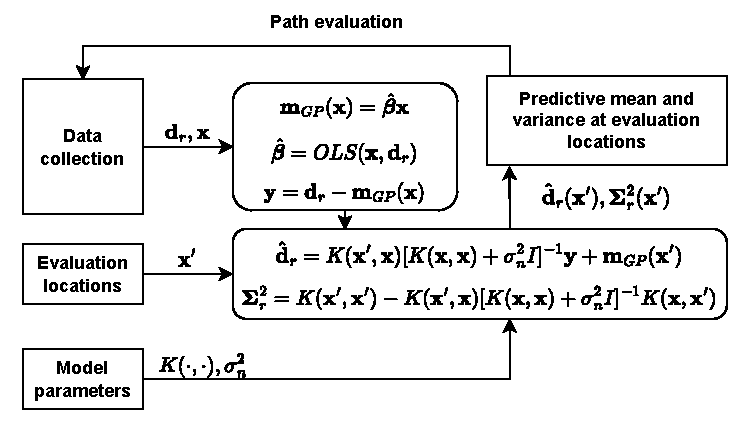
\includegraphics[width=0.95\textwidth]{figures/douromodelflow3-1.pdf}
    \caption{Flowchart representation of the model and method used in \textbf{paper B}, with $OLS(\cdot)$ beign the ordinary least squares, making $\mathbf{m}_{GP}(\mathbf{x})$ a linear regression. The vector $\mathbf{d}_r$ is the measurement vector, with input (position) vector $\mathbf{x}$, evaluation locations $\mathbf{x}'$, kernel $K(\cdot,\cdot)$, and nugget $\sigma^2_n$.}
    \label{fig:dmodflow}
\end{figure}

\subsubsection*{Gridded recursive GP}
A common \acrshort{gp} implementation\cite{fossum2019adaptive,stankiewicz2021adaptive,berget2018adaptive}, here termed \textit{gridded recursive GP}, is ingesting data piece wise, and in most cases assuming a static data field. This model is initiated by assigning the prior, $\mathbf{\mu}_0$, $\sigma_0$ to all grid cells. By creating the $F_k$-matrix, indicating the cells containing measurements at step $k$, the measurement function $f(\cdot)$ can be reduced to Equation \eqref{eq:recgridgp}.
\begin{align}
    \label{eq:recgridgp}
    y_k = F_k \mathbf{x}_k + \mathbf{\varepsilon}_k
\end{align}

The posterior is then calculated as a normal update-step, 
\begin{align}
    \label{eq:recgp2}
    \mathbf{\mu}_k &= \mathbf{\mu}_{k-1} + \Sigma_{k-1}F_k^{\intercal} (F_k\Sigma_{k-1}F_k^{\intercal} + \sigma_n^2 I)^{-1}(\mathbf{y}_k-F_k\mathbf{\mu}_{k-1}) \\
    \label{eq:recgp3}
    \Sigma_k &= \Sigma_{k-1} -  \Sigma_{k-1}F_k^{\intercal} (F_k\Sigma_{k-1}F_k^{\intercal} + \sigma_n^2 I)^{-1}F_k\Sigma_{k-1}^{\intercal},
\end{align}

using the $F$-matrix to augment the covariance matrix into the different covariance matrices in Equations \eqref{eq:mod_gp_pred}-\eqref{eq:mod_gp_pred3}. This formulation is made possible by gridding both the input and posterior, linking them in the same grid, similar to a Kalman Filter\cite{kalman1960new} without propagating the model or uncertainty in time. Attempts at adding noise for each update have been made\cite{berget2018adaptive} by augmenting Equation \eqref{eq:recgp3} to include the term $V\Sigma_0$, such that
\begin{align}
    \Sigma_k &= \Sigma_{k-1} -  \Sigma_{k-1}F_k^{\intercal} (F_k\Sigma_{k-1}F_k^{\intercal} + \sigma_n^2 I)^{-1}F_k\Sigma_{k-1}^{\intercal} + V\Sigma_0.
\end{align}

This is an attempt at taking the temporal variability of the ocean intro account, by increasing the covariance. Tuning of the constant $V$ has to be done in such a way that it mirrors the temporal decay of the measurements.  

